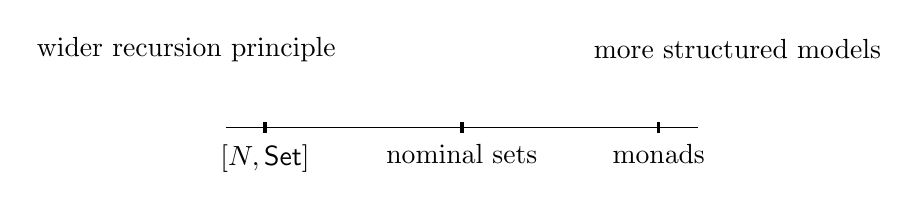
\begin{tikzpicture}
\draw[very thick] (-2.5,2pt)--(-2.5,-2pt) node [below] {$[\mathbb{N},\mathsf{Set}]$};
\draw[very thick] (0,2pt)--(0,-2pt) node [below] {nominal sets};
\draw[very thick] (2.5,2pt)--(2.5,-2pt) node [below] {monads};
\draw (-3,0) -- (3,0);
%\draw[->] (-3,1) edge node[above] {more structured models} (3,1) ;
%\draw[<-] (-3,-1) edge node[below] {wider recursion principle} (3,-1) ;
\node at (3.5,1) {more structured models};
\node at (-3.5,1) {wider recursion principle};
\end{tikzpicture}
